\section{Abs$<$ Sets\-Type, Measure, Cand\_\-Data\-Struct $>$ Class Template Reference}
\label{class_abs}\index{Abs@{Abs}}
Functor finding the negative border Bd- and/or the positive border Bd+ using the algorithm ABS.  


{\tt \#include $<$Abs.hxx$>$}

Inheritance diagram for Abs$<$ Sets\-Type, Measure, Cand\_\-Data\-Struct $>$::\begin{figure}[H]
\begin{center}
\leavevmode
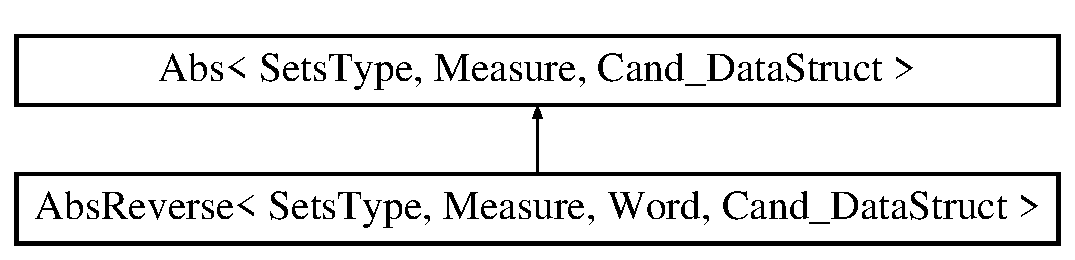
\includegraphics[height=2cm]{class_abs}
\end{center}
\end{figure}
\subsection*{Public Member Functions}
\begin{CompactItemize}
\item 
{\bf Abs} ()\label{class_abs_b9e1bb01229ec95da6b1a5f533dd7151}

\begin{CompactList}\small\item\em Constructor. \item\end{CompactList}\item 
{\bf $\sim$Abs} ()\label{class_abs_72d51b48cb02d0fbb3815d6f8dbf67e6}

\begin{CompactList}\small\item\em Destructor. \item\end{CompactList}\item 
template$<$class Init\-Functor, class Predicate, class Stop\-Iteration, class Output\-Bd\-P, class Output\-Bd\-N, class f$>$ void {\bf operator()} (Init\-Functor \&init, {\bf Predicate} \&pred, Stop\-Iteration $\ast$stop\-Dualization, Output\-Bd\-P $\ast$out\-Bd\-P, Output\-Bd\-N $\ast$out\-Bd\-N, f \&word\-To\-Set)
\begin{CompactList}\small\item\em Functor operator that executes the algorithm. \item\end{CompactList}\item 
template$<$class Init\-Functor, class Predicate, class Stop\-Iteration, class Output\-Bd\-P, class Output\-Bd\-N$>$ void {\bf operator()} (Init\-Functor \&init, {\bf Predicate} \&pred, Stop\-Iteration $\ast$stop\-Dualization, Output\-Bd\-P $\ast$out\-Bd\-P, Output\-Bd\-N $\ast$out\-Bd\-N)
\begin{CompactList}\small\item\em Functor operator that executes the algorithm. \item\end{CompactList}\end{CompactItemize}
\subsection*{Public Attributes}
\begin{CompactItemize}
\item 
bool {\bf verbose}\label{class_abs_346a3f491c7896baa2669113764d9fa7}

\begin{CompactList}\small\item\em {\bf Boolean}{\rm (p.\,\pageref{class_boolean})} to print to screen some informations during the execution (default false). \item\end{CompactList}\end{CompactItemize}
\subsection*{Protected Member Functions}
\begin{CompactItemize}
\item 
template$<$class Init\-Functor, class Predicate, class Stop\-Iteration, class Output\-Bd\-P, class Output\-Bd\-N, class Error, class f$>$ void {\bf execute\-Algorithm} (Init\-Functor \&init, {\bf Predicate} $\ast$pred, Stop\-Iteration $\ast$stop\-Dualization, Output\-Bd\-P $\ast$out\-Bd\-P, Output\-Bd\-N $\ast$out\-Bd\-N, Error $\ast$error, f \&word\-To\-Set)
\begin{CompactList}\small\item\em Execute the algorithm. \item\end{CompactList}\item 
template$<$class Predicate, class Error, class f$>$ int {\bf process\-Opt\-Gen\-Sub} ({\bf Predicate} $\ast$pred, {\bf PTree}$<$ Sets\-Type, Measure $>$ $\ast$compl\-Set, {\bf PTree}$<$ Sets\-Type, Measure $>$ $\ast$opt, {\bf PTree}$<$ Sets\-Type, Measure $>$ $\ast$tr, {\bf PTree}$<$ Sets\-Type, Measure $>$ $\ast$freq\-Tr, {\bf PTree}$<$ Sets\-Type, Measure $>$ $\ast$sub\-Set, int size, f \&word\-To\-Set, Error $\ast$error)
\begin{CompactList}\small\item\em Process the optimist positive border. \item\end{CompactList}\item 
void {\bf move\-Trans\-Freq} (vect\-UI $\ast$itemset, {\bf PTree}$<$ Sets\-Type, Measure $>$ $\ast$tr, {\bf PTree}$<$ Sets\-Type, Measure $>$ $\ast$freq\-Tr)
\begin{CompactList}\small\item\em Method that move a minimal transversal which have \char`\"{}generated\char`\"{} an interesting set from the set of minimal transversals to another set. \item\end{CompactList}\item 
template$<$class Predicate, class f$>$ int {\bf prune\-Candidates} ({\bf Predicate} $\ast$pred, {\bf PTree}$<$ Sets\-Type, Measure $>$ $\ast$tr, int level, deq\-It\-Cand \&last\-Bd\-NElem, f \&word\-To\-Set)
\begin{CompactList}\small\item\em Prune the not interesting elements generated by the levelwise exploration. \item\end{CompactList}\item 
void {\bf gen\-Cand} ({\bf PTree}$<$ Sets\-Type, Measure $>$ $\ast$sub\-Set, {\bf PTree}$<$ Sets\-Type, Measure $>$ $\ast$inbdp)
\begin{CompactList}\small\item\em Method generating the candidates of the levelwise exploration. \item\end{CompactList}\item 
template$<$class Predicate, class f$>$ void {\bf opt\-Approach} ({\bf Predicate} $\ast$pred, set$<$ {\bf PTree}$<$ Sets\-Type, Measure $>$ $>$ $\ast$opt\-It, int lvl, f \&word\-To\-Set)
\begin{CompactList}\small\item\em Method used to do the optimist approach based on \char`\"{}almost interesting\char`\"{} elements. \item\end{CompactList}\item 
template$<$class Predicate, class f$>$ int {\bf prune\-Candidates\-Opt} ({\bf Predicate} $\ast$pred, {\bf PTree}$<$ Sets\-Type, Measure $>$ $\ast$tr, f \&word\-To\-Set)
\begin{CompactList}\small\item\em \char`\"{}Prune\char`\"{} the interesting elements when exploring almost interesting elements. \item\end{CompactList}\end{CompactItemize}
\subsection*{Protected Attributes}
\begin{CompactItemize}
\item 
{\bf Apriori}$<$ Sets\-Type, Measure, Cand\_\-Data\-Struct $>$ {\bf apriori}\label{class_abs_e5143798f9be145d0712d57d553915c2}

\begin{CompactList}\small\item\em Algorithm apriori used for the bottom up initialization. \item\end{CompactList}\item 
Cand\_\-Data\-Struct $\ast$ {\bf bd\-N}\label{class_abs_84861429e931d82ff76926e5709ecd3f}

\begin{CompactList}\small\item\em Negative border. \item\end{CompactList}\item 
Cand\_\-Data\-Struct $\ast$ {\bf bd\-P}\label{class_abs_891257e049d0299337be5a48983a5297}

\begin{CompactList}\small\item\em Positive border. \item\end{CompactList}\end{CompactItemize}


\subsection{Detailed Description}
\subsubsection*{template$<$class Sets\-Type = int, class Measure = Boolean, class Cand\_\-Data\-Struct = PTree$<$Sets\-Type,Measure $>$$>$ class Abs$<$ Sets\-Type, Measure, Cand\_\-Data\-Struct $>$}

Functor finding the negative border Bd- and/or the positive border Bd+ using the algorithm ABS. 

The algorithme (\char`\"{}()\char`\"{} method)take in parameter: the initialisation functor, the predicate, the functor determining at which iteration the levelwise step is stop, the positive and/or negative borders (optional), the transformation function (optional).

The method execute\-Algorithm could be use to execute the algorithm. This method have another parameter to deal with \char`\"{}almost interesting elements\char`\"{} based on an error function passed i n parameter. These elements are considered as interesting during the iterations, and at the end they are used to do a top-down traversal of the search space to find the latests elements of Bd+.

The template parameter Sets\-Type represents the type of the elements of the set representation. The template parameter Measure is the type of the value eventually associated with the word of the language. The template parameter Cand\_\-Data\-Struct is the data structure type used by the algorithms to manipulate the candidates generated. 



\subsection{Member Function Documentation}
\index{Abs@{Abs}!executeAlgorithm@{executeAlgorithm}}
\index{executeAlgorithm@{executeAlgorithm}!Abs@{Abs}}
\subsubsection{\setlength{\rightskip}{0pt plus 5cm}template$<$class Sets\-Type, class Measure, class Cand\_\-Data\-Struct$>$ template$<$class Init\-Functor, class Predicate, class Stop\-Iteration, class Output\-Bd\-P, class Output\-Bd\-N, class Error, class f$>$ void {\bf Abs}$<$ Sets\-Type, Measure, Cand\_\-Data\-Struct $>$::execute\-Algorithm (Init\-Functor \& {\em init}, {\bf Predicate} $\ast$ {\em pred}, Stop\-Iteration $\ast$ {\em stop\-Dualization}, Output\-Bd\-P $\ast$ {\em out\-Bd\-P}, Output\-Bd\-N $\ast$ {\em out\-Bd\-N}, Error $\ast$ {\em error}, f \& {\em word\-To\-Set})\hspace{0.3cm}{\tt  [protected]}}\label{class_abs_33917103181d75de02278cb345c96c1a}


Execute the algorithm. 

\begin{Desc}
\item[Parameters:]
\begin{description}
\item[{\em init}]functor initializing the interesting items wrt predicate. \item[{\em pred}]the predicate \item[{\em stop\-Dualization}]functor determining when the apiori execution must stop \item[{\em bd\-P}]output the positive border in the given objet (must have a push\_\-back( container, measure ) method). \item[{\em bd\-N}]output the negative border in the given objet (must have a push\_\-back( container, measure ) method). \item[{\em error}]function processing if a not interesting element of the optimistic positive border is \char`\"{}almost interesting\char`\"{} \end{description}
\end{Desc}
\index{Abs@{Abs}!genCand@{genCand}}
\index{genCand@{genCand}!Abs@{Abs}}
\subsubsection{\setlength{\rightskip}{0pt plus 5cm}template$<$class Sets\-Type, class Measure, class Cand\_\-Data\-Struct$>$ void {\bf Abs}$<$ Sets\-Type, Measure, Cand\_\-Data\-Struct $>$::gen\-Cand ({\bf PTree}$<$ Sets\-Type, Measure $>$ $\ast$ {\em sub\-Set}, {\bf PTree}$<$ Sets\-Type, Measure $>$ $\ast$ {\em inbdp})\hspace{0.3cm}{\tt  [protected]}}\label{class_abs_41ebb2a6cc990dee19092f6ca21effa8}


Method generating the candidates of the levelwise exploration. 

Actually, this method delete all the subsets generated when processing the optimistic positive border which are included into one element of Bd+.

\begin{Desc}
\item[Parameters:]
\begin{description}
\item[{\em sub\-Set}]subsets of size k+1 of the not interesting elements find in the optimistic positive border. \item[{\em inbdp}]the positive border (all the elements of Bd+ found until the current iteration) \end{description}
\end{Desc}
\index{Abs@{Abs}!moveTransFreq@{moveTransFreq}}
\index{moveTransFreq@{moveTransFreq}!Abs@{Abs}}
\subsubsection{\setlength{\rightskip}{0pt plus 5cm}template$<$class Sets\-Type, class Measure, class Cand\_\-Data\-Struct$>$ void {\bf Abs}$<$ Sets\-Type, Measure, Cand\_\-Data\-Struct $>$::move\-Trans\-Freq (vect\-UI $\ast$ {\em itemset}, {\bf PTree}$<$ Sets\-Type, Measure $>$ $\ast$ {\em tr}, {\bf PTree}$<$ Sets\-Type, Measure $>$ $\ast$ {\em freq\-Tr})\hspace{0.3cm}{\tt  [protected]}}\label{class_abs_4069503604644bb7ddb2404a47098663}


Method that move a minimal transversal which have \char`\"{}generated\char`\"{} an interesting set from the set of minimal transversals to another set. 

\begin{Desc}
\item[Parameters:]
\begin{description}
\item[{\em itemset}]set wich have generated an interesting element \item[{\em tr}]set of the minimal transversals (those which have generated not interesting elements) \item[{\em freq\-Tr}]set of the minmal tranversals which have generated an interesting elements \end{description}
\end{Desc}
\index{Abs@{Abs}!operator()@{operator()}}
\index{operator()@{operator()}!Abs@{Abs}}
\subsubsection{\setlength{\rightskip}{0pt plus 5cm}template$<$class Sets\-Type = int, class Measure = Boolean, class Cand\_\-Data\-Struct = PTree$<$Sets\-Type,Measure $>$$>$ template$<$class Init\-Functor, class Predicate, class Stop\-Iteration, class Output\-Bd\-P, class Output\-Bd\-N$>$ void {\bf Abs}$<$ Sets\-Type, Measure, Cand\_\-Data\-Struct $>$::operator() (Init\-Functor \& {\em init}, {\bf Predicate} \& {\em pred}, Stop\-Iteration $\ast$ {\em stop\-Dualization}, Output\-Bd\-P $\ast$ {\em out\-Bd\-P}, Output\-Bd\-N $\ast$ {\em out\-Bd\-N})\hspace{0.3cm}{\tt  [inline]}}\label{class_abs_1cb8186e971cbb42b54d29bab5ba1e01}


Functor operator that executes the algorithm. 

\begin{Desc}
\item[Parameters:]
\begin{description}
\item[{\em init}]functor initializing the interesting items wrt predicate. \item[{\em pred}]the predicate \item[{\em stop\-Dualization}]functor determining when the apiori execution must stop \item[{\em bd\-P}]output the positive border in the given objet (must have a push\_\-back( container, measure ) method). \item[{\em bd\-N}]output the negative border in the given objet (must have a push\_\-back( container, measure ) method). \end{description}
\end{Desc}


Reimplemented in {\bf Abs\-Reverse$<$ Sets\-Type, Measure, Word, Cand\_\-Data\-Struct $>$} {\rm (p.\,\pageref{class_abs_reverse_783d932854ce93bd14518406996d8090})}.\index{Abs@{Abs}!operator()@{operator()}}
\index{operator()@{operator()}!Abs@{Abs}}
\subsubsection{\setlength{\rightskip}{0pt plus 5cm}template$<$class Sets\-Type = int, class Measure = Boolean, class Cand\_\-Data\-Struct = PTree$<$Sets\-Type,Measure $>$$>$ template$<$class Init\-Functor, class Predicate, class Stop\-Iteration, class Output\-Bd\-P, class Output\-Bd\-N, class f$>$ void {\bf Abs}$<$ Sets\-Type, Measure, Cand\_\-Data\-Struct $>$::operator() (Init\-Functor \& {\em init}, {\bf Predicate} \& {\em pred}, Stop\-Iteration $\ast$ {\em stop\-Dualization}, Output\-Bd\-P $\ast$ {\em out\-Bd\-P}, Output\-Bd\-N $\ast$ {\em out\-Bd\-N}, f \& {\em word\-To\-Set})\hspace{0.3cm}{\tt  [inline]}}\label{class_abs_991fe73b7db6f50b75e434631187ec9a}


Functor operator that executes the algorithm. 

\begin{Desc}
\item[Parameters:]
\begin{description}
\item[{\em init}]functor initializing the interesting items wrt predicate \item[{\em pred}]the predicate \item[{\em stop\-Dualization}]functor determining when the apiori execution must stop \item[{\em bd\-P}]output the positive border in the given objet (must have a push\_\-back( container, measure ) method). \item[{\em bd\-N}]output the negative border in the given objet (must have a push\_\-back( container, measure ) method). \item[{\em word\-Toset}]transformation function \end{description}
\end{Desc}


Reimplemented in {\bf Abs\-Reverse$<$ Sets\-Type, Measure, Word, Cand\_\-Data\-Struct $>$} {\rm (p.\,\pageref{class_abs_reverse_d4e6aa7d0f2e50db5d5e75ab5801fd51})}.\index{Abs@{Abs}!optApproach@{optApproach}}
\index{optApproach@{optApproach}!Abs@{Abs}}
\subsubsection{\setlength{\rightskip}{0pt plus 5cm}template$<$class Sets\-Type, class Measure, class Cand\_\-Data\-Struct$>$ template$<$class Predicate, class f$>$ void {\bf Abs}$<$ Sets\-Type, Measure, Cand\_\-Data\-Struct $>$::opt\-Approach ({\bf Predicate} $\ast$ {\em pred}, set$<$ {\bf PTree}$<$ Sets\-Type, Measure $>$ $>$ $\ast$ {\em opt\-It}, int {\em lvl}, f \& {\em word\-To\-Set})\hspace{0.3cm}{\tt  [protected]}}\label{class_abs_61298c6d5b7e4ff5192b2a68c52b701a}


Method used to do the optimist approach based on \char`\"{}almost interesting\char`\"{} elements. 

From a set of sets in parameter, it founds all the maximals interesting sets of the sub lattice until a given level. the exploration of the search space id done level by level.

\begin{Desc}
\item[Parameters:]
\begin{description}
\item[{\em pred}]the predicate \item[{\em opt\-It}]set containing the almost interesting elements (strored by size) \item[{\em lvl}]the \char`\"{}smallest\char`\"{} level to explore \item[{\em word\-Toset}]transformation function \end{description}
\end{Desc}
\index{Abs@{Abs}!processOptGenSub@{processOptGenSub}}
\index{processOptGenSub@{processOptGenSub}!Abs@{Abs}}
\subsubsection{\setlength{\rightskip}{0pt plus 5cm}template$<$class Sets\-Type, class Measure, class Cand\_\-Data\-Struct$>$ template$<$class Predicate, class Error, class f$>$ int {\bf Abs}$<$ Sets\-Type, Measure, Cand\_\-Data\-Struct $>$::process\-Opt\-Gen\-Sub ({\bf Predicate} $\ast$ {\em pred}, {\bf PTree}$<$ Sets\-Type, Measure $>$ $\ast$ {\em compl\-Set}, {\bf PTree}$<$ Sets\-Type, Measure $>$ $\ast$ {\em opt}, {\bf PTree}$<$ Sets\-Type, Measure $>$ $\ast$ {\em tr}, {\bf PTree}$<$ Sets\-Type, Measure $>$ $\ast$ {\em freq\-Tr}, {\bf PTree}$<$ Sets\-Type, Measure $>$ $\ast$ {\em sub\-Set}, int {\em size}, f \& {\em word\-To\-Set}, Error $\ast$ {\em error})\hspace{0.3cm}{\tt  [protected]}}\label{class_abs_18e3c9003dca0c22177631287ce60aa5}


Process the optimist positive border. 

All the interesting sets update Bd+ and the subests of the not interesting sets are generated. If the \char`\"{}almost interesting\char`\"{} elements are studied, this method save these elements in a particular data structure. To optimize the minimal transversal computation, minimal transversals which have generated an interesting element are stored separately.

\begin{Desc}
\item[Parameters:]
\begin{description}
\item[{\em pred}]the predicate \item[{\em compl\-Set}]set of complements of the minimal transversals in the current iteration \item[{\em opt}]set used to store the almost interesting elments (not necessarly used) \item[{\em tr}]set of the minimal transversals find until the current iteration \item[{\em freqtr}]set of the minimal transversals find until the current iteration and which have generated an interesting element \item[{\em sub\-Set}]strore the subsets of size k (current level of the levelwise approach) of the not interesting elements fond in the optimistic positive border \item[{\em size}]current level of the levelwise approach \item[{\em word\-Toset}]transformation function \item[{\em error}]function processing if a not interesting element of the optimistic positive border is \char`\"{}almost interesting\char`\"{} \end{description}
\end{Desc}
\index{Abs@{Abs}!pruneCandidates@{pruneCandidates}}
\index{pruneCandidates@{pruneCandidates}!Abs@{Abs}}
\subsubsection{\setlength{\rightskip}{0pt plus 5cm}template$<$class Sets\-Type, class Measure, class Cand\_\-Data\-Struct$>$ template$<$class Predicate, class f$>$ int {\bf Abs}$<$ Sets\-Type, Measure, Cand\_\-Data\-Struct $>$::prune\-Candidates ({\bf Predicate} $\ast$ {\em pred}, {\bf PTree}$<$ Sets\-Type, Measure $>$ $\ast$ {\em tr}, int {\em level}, deq\-It\-Cand \& {\em last\-Bd\-NElem}, f \& {\em word\-To\-Set})\hspace{0.3cm}{\tt  [protected]}}\label{class_abs_46ecf54530c316a639b3533386af9d4b}


Prune the not interesting elements generated by the levelwise exploration. 

\begin{Desc}
\item[Parameters:]
\begin{description}
\item[{\em pred}]the predicate \item[{\em tr}]set of the candidates generated by the levelwise exploration \item[{\em level}]current level of the levelwise exploration \item[{\em last\-Bd\-NElem}]elements (iterators on) of the negative border found in the current iteration \item[{\em word\-Toset}]transformation function \end{description}
\end{Desc}
\index{Abs@{Abs}!pruneCandidatesOpt@{pruneCandidatesOpt}}
\index{pruneCandidatesOpt@{pruneCandidatesOpt}!Abs@{Abs}}
\subsubsection{\setlength{\rightskip}{0pt plus 5cm}template$<$class Sets\-Type, class Measure, class Cand\_\-Data\-Struct$>$ template$<$class Predicate, class f$>$ int {\bf Abs}$<$ Sets\-Type, Measure, Cand\_\-Data\-Struct $>$::prune\-Candidates\-Opt ({\bf Predicate} $\ast$ {\em pred}, {\bf PTree}$<$ Sets\-Type, Measure $>$ $\ast$ {\em tr}, f \& {\em word\-To\-Set})\hspace{0.3cm}{\tt  [protected]}}\label{class_abs_9756459bbd5a86de592167e310c576fa}


\char`\"{}Prune\char`\"{} the interesting elements when exploring almost interesting elements. 

The interesting elements are pruned for further exploration but stored in the positive border.

\begin{Desc}
\item[Parameters:]
\begin{description}
\item[{\em pred}]the predicate \item[{\em tr}]the set of candidates generated by the exploration \item[{\em word\-Toset}]transformation function \end{description}
\end{Desc}


The documentation for this class was generated from the following file:\begin{CompactItemize}
\item 
F:/i\-Zi/algorithms/Abs.hxx\end{CompactItemize}
